\chapter{变分法}
    前面的定态微扰论很方便, 也很精确, 但是我们还是要事先求出未微扰的波函数, 然后代入公式计算。\footnote{做{\itshape Griffiths}的习题你就知道有多痛苦了}
    而下面要介绍的变分法就是在我们完全不知道, 也不用知道波函数的情况下较为近似的给出基态能量大小。当然它也可以进一步推广去求激发态, 现在也有很多计算物理算法是基于此原理的

    \section{基本原理}
    我们假设体系的基态能量为$E_{gs}$, 基态波函数为$\ket{\psi_{0}}$。方便起见, 先考虑离散谱非简并的系统, $\hat{H}$本征矢构成的正交完备基设为$\{\ket{\psi_n}\}$。\footnote{对于变分法, 简并和非简并情况是可以统一处理的}

    现在我们考虑态空间$\mathscr{E}$中的\uwave{任意}一个归一化的态矢量$\ket{\psi}$, 可以展开为:
    \[\ket{\psi}=\sum_{n=0}^{\infty}c_n\ket{\psi_n},\quad\sum_{n=0}^{\infty}|c_n|^2=1\]
    在没有求解方程之前, 我们完全有理由认为这个态矢量为真实的解, 我们求一下在这个态下的能量平均值:
    \begin{align*}
        \braket{\psi|\hat{H}|\psi}&=\sum_{n=0}^{\infty}c_n\braket{\psi|\hat{H}|\psi_n}=\sum_{n=0}^{\infty}E_nc_n\braket{\psi|\psi_n}\\
        &=\sum_{n=0}^{\infty}|c_n|^2E_n\geq E_{gs}\sum_{n=0}^{\infty}|c_n|^2=E_{gs}
    \end{align*}
    更一般的情况下我们不要求$\ket{\psi}$本身是归一化的, 我们先给它归一化后再代入计算便可以得到更为通用的形式:
    \begin{equation}
        \label{eq:8.1}
        \boxed{
            E_{gs}=\mathrm{min}\left[\frac{\braket{\psi|\hat{H}|\psi}}{\braket{\psi|\psi}}\right],\quad\psi\in\mathscr{E}
        }
    \end{equation}

    上面这个式子可以理解为粒子找遍了态空间中所有可取的波函数, 最后取了一个可以使得能量最小的波函数作为基态波函数, 是不是有点最小作用量原理的味道了?那这又是怎么和变分联系起来的呢?
    我们刚才只是证明了它是定态薛定谔方程的必要条件, 现在验证一下充分性。

    我们把$\ref{eq:8.1}$的右边看成是关于$\ket{\psi}$的\uwave{泛函}, 记作$E[\psi]$。基态波函数的选取使得$E[\psi]$取极小值, 或者说一阶变分$\delta E[\psi_0]=0$:
    \begin{equation*}
        \delta E[\psi]=\delta\frac{\braket{\psi|\hat{H}|\psi}}{\braket{\psi|\psi}}
        =\frac{\braket{\psi|\psi}\delta \braket{\psi|\hat{H}|\psi}-\braket{\psi|\hat{H}|\psi}\delta \braket{\psi|\psi}}{\braket{\psi|\psi}^2}
    \end{equation*}
    上面的方程在波函数取正确的基态$\ket{\psi_0}$时为0, 记$E_{gs}=E[\psi_0]$:
    \[\braket{\delta\psi|\hat{H}|\psi_0}+\braket{\psi_0|\hat{H}|\delta\psi}=E_{gs}\left(\braket{\psi_0|\delta\psi}+\braket{\delta\psi|\psi_0}\right)\]
    $E_gs$是常数, 所以可以直接纳入braket里面, 移项整理后得到:
    \[\mathrm{Re}\left[\Braket{\delta\psi|\hat{H}-E_{gs}|\psi_0}\right]=0\]
    
    和我们推导Euler-Lagrange方程是所做的一样, 上式要对任意的$\delta\psi$成立, 只能有:
    $$\hat{H}\ket{\psi_0}=E_{gs}\ket{\psi_0}$$
    而这正是基态的定态薛定谔方程!

    变分问题我们近似的解的话思路就是找一堆可能的函数簇$$\{\psi(x;\alpha_1,\alpha_2,\cdots,\alpha_n)\}$$其中$\alpha_i$表示参数, 我们称之为\uwave{试探函数}。
    对于每个试探函数我们算一个$E[\psi]$, 我们便确定了基态能量的一个上界, 而且这个上界会越来越小, 越来越趋近于真值, 我们最终计算得到的能量泛函肯定是$\alpha_i$的函数,
    我们最后取一个最小的上界作为$E_gs$的近似值就好, 也就是说我们还要解方程组:
    \[\frac{\partial}{\partial\alpha_i}E_\psi[\alpha_1,\alpha_2,\cdots,\alpha_n]=0,\quad (i=1,2,\cdots,n)\]

    我们选取的试探函数参数越多, 形式和$\psi_0$越接近, 近似效果就会越好, 最后看一个例子。
    \begin{example}{谐振子}
        谐振子问题$V(x)=\frac{1}{2}m\omega^2x^2$是可以精确求解的, 我们这里用变分法估计一下它的基态能量上界。试探函数一般取为下面的高斯函数:
        \begin{equation}
            \label{eq:8.2}
            \psi(x;b)=Ae^{-bx^2}\xleftarrow[]{normalized}A=\left(\frac{2b}{\pi}\right)^{1/4}
        \end{equation}
    不难计算得到$\braket{\psi|\hat{H}|\psi}$:
    \begin{equation*}
        \langle T\rangle=-\frac{\hbar^{2}}{2 m}|A|^{2} \int_{-\infty}^{\infty} e^{-b \cdot x^{2}} \frac{d^{2}}{d x^{2}}\left(e^{-b . x^{2}}\right) d x=\frac{\hbar^{2} b}{2 m}
    \end{equation*}
    \begin{equation*}
        \langle V\rangle=\frac{1}{2} m \omega^{2}|A|^{2} \int_{-\infty}^{\infty} e^{-2 b x^{2}} x^{2} d x=\frac{m \omega^{2}}{8 b}
    \end{equation*}
    \begin{equation*}
        \langle H\rangle=\frac{\hbar^{2} b}{2 m}+\frac{m \omega^{2}}{8 b}
    \end{equation*}
    我们选取参数$b$得到最小的上界:
    \begin{equation*}
        \frac{\partial}{\partial b}\braket{H}=\frac{\hbar^2}{2m}-\frac{m\omega^2}{8b^2}=0\Rightarrow b=\frac{m\omega}{2\hbar}
    \end{equation*}
    这样我们便得到:
    \begin{equation*}
        E_{gs}\leq\frac{1}{2}\omega\hbar
    \end{equation*}
    我们得到的不只是上界还是上确界!究其原因还是因为我们试探函数取的好, 基态波函数恰好就是\ref{eq:8.2}的形式。
    \end{example}

    变分法其实也能用于激发态的求解, 但是用起来要复杂一些, 所以很少使用。
    \begin{theorem}{变分法估计第一激发态}
        如果$\braket{\psi|\psi_{gs}}=0$(normalized), 那么$\braket{H}_\psi\geq E_{fe}$
    \end{theorem}
    
    这个定理的证明和前面的一个套路, 这里就直接略去了。
    
    上面的定理的关键在于去找寻与基态正交的试探波函数, 而由于我们有时候甚至不知道基态波函数长什么样, 所以用起来很难。但是当系统具有某种对称性时, 也就是说存在一个厄米算符$\hat{A}$, 有
    $\left[\hat{A},\hat{H}\right]=0$, 那么各级波函数可以取为他们的共同本征矢, 我们若是知道了$A\psi_{gs}=\lambda\psi_{gs}$, 那么根据厄米性, $A$的本征值为$\nu\neq\lambda$对应
    的本征矢一定与$\psi_{gs}$正交。比如氢原子, $\hat A$便是$J^2$, 角量子数$\ell=0$说基态取值, 那么我们选取$J^2$的本征值为$\ell=1$的本征矢去试探便可以估计$E_{fs}$的上界。
    
    \section{氦原子的基态能量}
    首先复习一下氦原子的哈密顿量:
    \begin{equation}
        H=-\frac{\hbar^{2}}{2 m}\left(\nabla_{1}^{2}+\nabla_{2}^{2}\right)-\frac{e^{2}}{4 \pi \epsilon_{0}}\left(\frac{2}{r_{1}}+\frac{2}{r_{2}}-\frac{1}{\left|\mathbf{r}_{1}-\mathbf{r}_{2}\right|}\right)
    \end{equation}
    难以处理的地方在于电子之间的相互作用势能:
    \begin{equation}
        V_{ee}=\frac{e^{2}}{4 \pi \epsilon_{0}} \frac{1}{\left|\mathbf{r}_{1}-\mathbf{r}_{2}\right|}
    \end{equation}
    我们前面已经说过, 如果不考虑这个势能, 那么基态波函数就可以写为\footnote{参考\ref{eq:4.41}, 注意这里氦原子核电荷为2, 即$Z=2$,$a\to\frac{a}{2}$}:
    \begin{equation}
        \label{eq:8.5}
        \psi_{0}\left(\mathbf{r}_{1}, \mathbf{r}_{2}\right) \equiv \psi_{100}\left(\mathbf{r}_{1}\right) \psi_{100}\left(\mathbf{r}_{2}\right)=\frac{8}{\pi a^{3}} e^{-2\left(r_{1}+r_{2}\right) / a}
    \end{equation}
    
    或许有疑问电子是费米子, 他的态按照我们前面说的应该是反对称的才对啊?注意这里不要忘了电子的自旋态, 这里波函数$\psi_0$对称, 而他们的自旋态是singlet反对称的。

    上面的这个非常粗略的波函数是略去$V_{ee}$后哈密顿量的本征矢, 给出的基态能量不难发现为$2\times 2^2 E_1=8E_1\approx\SI{-109}{eV}$, 而实验上的结果为$\SI{-78.975}{eV}$。看来完全忽略电子之间的相互作用是不可行的, 但是这给了我们灵感, 
    利用变分法, 或许我们可以利用\ref{eq:8.5}计算一个基态能量的上界。

    把$H$分解为$H^0+V_{ee}$, 前面已说过$H^0\psi_0=8E_1\psi_0$, 所以我们关键是去求$\braket{V_{ee}}$:
    \begin{equation}
        \label{eq:8.6}
        \braket{V_{ee}}=\left(\frac{e^2}{4\pi\varepsilon_0}\right)^2\left(\frac{8}{\pi a^3}\right)^2\underbrace{\int\frac{e^{-4(r_1+r_2)/a}}{|\mathbf{r}_1-\mathbf{r}_2|}d^3r_1d^3r_2}_{I}
    \end{equation}
    
    为了计算这个积分, 我们先对$\mathbf{r}_1$积分, 注意这里的积分含义, 是在$\mathbf{r}_2$确定之后对$\mathbf{r}_1$全空间积分, 所以这个时候我们就可以取一个球坐标系去计算,
    将这个球坐标系的$z$轴方向取为$\mathbf{r}_2$方向, 其余定义与通常的球坐标系一致, 我们便可以化简得到:

    \begin{align*}
        I&=\int d^3r_2e^{-4r_2/a}\int^{\infty}_{0}dr_1 r_1^2e^{-4r_1/a}\int_0^\pi\frac{\sin\theta d\theta}{\sqrt{r_1^2+r_2^2-2r_1r_2\cos\theta}}\int_0^{2\pi}d\phi\\
        &=2\pi\int d^3r_2e^{-4r_2/a}\int^{\infty}_{0}dr_1 \frac{r_1}{r_2}e^{-4r_1/a}\mathrm{min}\{r_1,r_2\}\\
        &=\frac{\pi a^{3}}{8}\iiint\left[1-\left(1+\frac{2 r_{2}}{a}\right) e^{-4 r_{2} / a}\right] e^{-4 r_{2} / a} r_{2} \sin \theta_{2} d r_{2} d \theta_{2} d \phi_{2}\\
        &=\frac{5\pi^2a^5}{256}
    \end{align*} 
    再代入到\ref{eq:8.6}最终得到:
    \[\braket{V_{ee}}=\frac{5}{4a}\left(\frac{e^2}{4\pi\varepsilon_0}\right)=-\frac{5}{2}E_1\approx\SI[]{34}{eV}\]
    能量上界便为$\SI[]{-109}{eV}-(\SI[]{-34}{eV})=\SI[]{-75}{eV}$.

    到这儿还不是变分法的极限, 我们前面不是都是用的一簇函数吗?这里只用了一个波函数去估计上界, 所以差异还是比较大。实际上从结果上来看, \ref{eq:8.5}应该和真实的
    基态波函数差不多了, 我们只需要再加一点点改进就能让上界更加逼近于真实值。注意到\ref{eq:8.5}这个式子蕴含着\textbf{每个电子感受到的原子核吸引为电荷$2e$}, 但是
    实际上肯定不是这样, 另一个电子会排斥它, 或者说“中和”掉了原子核的正电荷, 导致最后电子感受到的原子核的核电荷数$Z$必然小于2, 那我们不妨直接把$Z$当作是参数写下这样的一簇试探波函数:
    \begin{equation}
        \label{eq:8.7}
        \psi_{1}\left(\mathbf{r}_{1}, \mathbf{r}_{2}\right) \equiv \frac{Z^{3}}{\pi a^{3}} e^{-Z\left(r_{1}+r_{2}\right) / a}
    \end{equation}
    
    这个式子就蕴含着我们刚才的思想, 由于电子之间的相互作用, 现在等效来看原子核的核电荷数$Z<2$。然后我们利用这一簇试探函数求$\braket{H}$。

    我们先再次重组一下哈密顿量:
    \begin{equation}
        \label{eq:8.8}
        \begin{aligned}
            H &=H_1+H_2\\
            & -\frac{\hbar^{2}}{2 m}\left(\nabla_{1}^{2}+\nabla_{2}^{2}\right)-\frac{e^{2}}{4 \pi \epsilon_{0}}\left(\frac{Z}{r_{1}}+\frac{Z}{r_{2}}\right) \\
            & +\frac{e^{2}}{4 \pi \epsilon_{0}}\left(\frac{(Z-2)}{r_{1}}+\frac{(Z-2)}{r_{2}}+\frac{1}{\left|\mathbf{r}_{1}-\mathbf{r}_{2}\right|}\right)
        \end{aligned}
    \end{equation}
    类比后不难知道\ref{eq:8.7}中有$H_1\psi_0=2Z^2E_1$, 所以
    \begin{equation}
        \label{eq:8.9}
        \langle H\rangle=2 Z^{2} E_{1}+2(Z-2)\left(\frac{e^{2}}{4 \pi \epsilon_{0}}\right)\Braket{\frac{1}{r}}+\left\langle V_{e e}\right\rangle
    \end{equation}
    根据上一章的\ref{eq:7.16}, 我们知道$\braket{r^{-1}}=Z/a$。\footnote{\ref{eq:8.8}中的$H_1$和氢原子的哈密顿量相比较只是$e\to Ze$的区别, 解的数学形式完全相同, 根据$a$和$e$之间的依赖关系, 我们只需要将$a$替换成$a/Z$就好了。}
    
    $V_{ee}$的求解和前面完全一样, 现在我们只需要把解中的$a$替换为$2a/Z $就好(本来我们之前就是按照$Z=2$去求的, 相当于$a$先替换为了$a/2$, 所以这里不足为奇)。
    \[\left\langle V_{e e}\right\rangle=\frac{5 Z}{8 a}\left(\frac{e^{2}}{4 \pi \epsilon_{0}}\right)=-\frac{5 Z}{4} E_{1}\]
    再根据\ref{eq:8.9}得:
    \[\langle H\rangle=\left[2 Z^{2}-4 Z(Z-2)-(5 / 4) Z\right] E_{1}=\left[-2 Z^{2}+(27 / 4) Z\right] E_{1}\]
    
    最后根据变分法我们得到$Z=\frac{27}{16}$时确定了一个最小上界为$\braket{H}=\SI[]{-77.5}{eV}$。这和我们实验仅仅相差不到$\SI[]{1.5}{eV}$

    \section{$\ce{H2^+}$ 和 $\ce{H2}$}
    这一节中我们将会看到量子化学家是如何将变分原理用于键长和键能的估计的。
    本节还会略去很多计算过程, 仅保留一些计算提示和计算结果, 相信我, 它们并不太复杂。
    \subsection*{$\ce{H2^+}$}
    这个情况简单一些, 类似于限制性三体问题, 我们假设两个质子是不动的($\ce{H}$原子核中的中子对我们的分析没有任何影响), 进一步假设两个质子之间的距离是$R$, 
    这其实对应化学键键长。那么哈密顿量可以写为:
    \begin{equation}
        H=-\frac{\hbar^2}{2m}\nabla^2-\frac{e^2}{4\pi\varepsilon_0}\left(\frac{1}{r}+\frac{1}{r^\prime}\right)+\bcancel{\frac{e^2}{4\pi\varepsilon_0R}}
    \end{equation}
    最后一项在$R$取得定值时是常数, 所以们先把它给去掉, 最后把这个能量加上来就好。式中的$r$和$r^\prime$是电子与两个质子之间的距离。

    我们首先考虑一个基态氢原子, 电子的波函数为:
    \[\psi_0(\mathbf{r})=\frac{1}{\sqrt{\pi a^3}}e^{-r/a}\]
    
    化学家常常把这个称为电子的“\uwave{轨道}”, 现在考虑另一个质子, 只要$R$与$a$相比不是太小, 我们就可以认为电子的轨道没有变化, 电子相对于另一个质子应该
    有相同的轨道$\psi(r^\prime)$, 我们把这两个轨道进行线性组合, 认为是新的电子轨道, 当然根据前面的说法, 只有在$R$与$a$相比不是太小时我们才能线性的这么做:
    \begin{equation}
        \psi = A\psi_0(\mathbf{r})+B\psi(\mathbf{r^\prime})
    \end{equation}
    当然, 这里$r$和$r^\prime$可不是独立的两个坐标, 我们最终要把他们在同一个坐标系下表示。

    化学家称这种方法为\textbf{原子轨道线性组合(LCAO\footnote{\textbf{l}inear \textbf{c}ombination of \textbf{a}tomic \textbf{o}rbitals})}。从物理上看
    就是有一定逻辑的猜出了试探波函数。根据对称性, 两个质子应该有同等的地位, 所以我们进一步认为$A=B$:
    \begin{equation}
        \label{eq:8.12}
        \psi = A\left[\psi_0(\mathbf{r})+\psi(\mathbf{r^\prime})\right]
    \end{equation}
    首先就是要进行归一化得到$A$:
    \begin{equation}
        \begin{aligned}
            1= & \int|\psi|^{2} d^{3} \mathbf{r}=|A|^{2}\left[\int \psi_{0}(r)^{2} d^{3} \mathbf{r}\right. \\
            & \left.+\int \psi_{0}\left(r^{\prime}\right)^{2} d^{3} \mathbf{r}+2 \int \psi_{0}(r) \psi_{0}\left(r^{\prime}\right) d^{3} \mathbf{r}\right]
        \end{aligned}
    \end{equation}
    括号里面前两项都好说, 都是1, 难算的在后面一个积分, 选取合适的坐标系, 将两个质子安排在$z$轴上并用球坐标计算:
    \begin{equation}
        \label{eq:8.14}
        \begin{aligned}
            I &\equiv\left\langle\psi_{0}(r) \mid \psi_{0}\left(r^{\prime}\right)\right\rangle=\frac{1}{\pi a^{3}} \int e^{-\left(r+r^{\prime}\right) / a} d^{3} \mathbf{r}\\
            &=e^{-R / a}\left[1+\left(\frac{R}{a}\right)+\frac{1}{3}\left(\frac{R}{a}\right)^{2}\right]
        \end{aligned}
    \end{equation}
    最终得到:
    \[|A|^{2}=\frac{1}{2(1+I)}\]
    下面就开始根据变分法计算基态能量的上界了, 首先注意到下面两个式子:
    \begin{equation}
        \label{eq:8.15}
        \begin{aligned}
        &\left(-\frac{\hbar^{2}}{2 m} \nabla^{2}-\frac{e^{2}}{4 \pi \epsilon_{0}} \frac{1}{r}\right) \psi_{0}(r)=E_{1} \psi_{0}(r)\\
        &\left(-\frac{\hbar^{2}}{2 m} \nabla^{2}-\frac{e^{2}}{4 \pi \epsilon_{0}} \frac{1}{r^\prime}\right) \psi_{0}(r^\prime)=E_{1} \psi_{0}(r^\prime)
        \end{aligned}
    \end{equation}
    那么便有:
    \begin{equation}
        \begin{aligned}
            H \psi & =A\left[-\frac{\hbar^{2}}{2 m} \nabla^{2}-\frac{e^{2}}{4 \pi \epsilon_{0}}\left(\frac{1}{r}+\frac{1}{r^{\prime}}\right)\right]\left[\psi_{0}(r)+\psi_{0}\left(r^{\prime}\right)\right] \\
            & =E_{1} \psi-A\left(\frac{e^{2}}{4 \pi \epsilon_{0}}\right)\left[\frac{1}{r^{\prime}} \psi_{0}(r)+\frac{1}{r} \psi_{0}\left(r^{\prime}\right)\right] 
        \end{aligned}
    \end{equation}
    注意到:
    \begin{equation}
        \label{eq:8.17}
        \begin{aligned}
            &\Braket{\psi_0(r)|\frac{1}{r^\prime}|\psi_0(r^\prime)}=\Braket{\psi_0(r^\prime)|\frac{1}{r}|\psi_0(r)}\\
            &\Braket{\psi_0(r)|\frac{1}{r^\prime}|\psi_0(r)}=\Braket{\psi_0(r^\prime)|\frac{1}{r}|\psi_0(r^\prime)}
        \end{aligned}
    \end{equation}
    
    因为这只是相当于积分变量的重新命名$r\leftrightarrow r^\prime$.便有:
    \begin{equation*}
        \langle H\rangle=E_{1}-2|A|^{2}\left(\frac{e^{2}}{4 \pi \epsilon_{0}}\right)\left[\underbrace{\left\langle\psi_{0}(r)\left|\frac{1}{r^{\prime}}\right| \psi_{0}(r)\right\rangle}_D+\underbrace{ \left\langle\psi_{0}(r)\left|\frac{1}{r}\right| \psi_{0}\left(r^{\prime}\right)\right\rangle}_X\right]
    \end{equation*}
    然后又是两个比较难算的积分, 不过只要知道$I$怎么计算, 这两个也就简单了:
    \begin{equation}
        \label{eq:8.18}
        D=\frac{a}{R}-\left(1+\frac{a}{R}\right) e^{-2 R / a}
    \end{equation}
    \begin{equation}
        \label{eq:8.19}
        X=\left(1+\frac{R}{a}\right) e^{-R / a}
    \end{equation}
    终于我们计算出了$\braket{H}$, 不过别忘了之前我们作为常数在之前计算中忽略的项, 也就是质子之间的电势能, 这里加上来\footnote{第二项实际上可以写为$-\frac{2a}{R}E_1$}:
    \begin{equation}
        \label{eq:8.20}
        E_{gs}\leq\left[1+2 \frac{(D+X)}{(1+I)}\right] E_{1}+\frac{e^{2}}{4 \pi \epsilon_{0}} \frac{1}{R}
    \end{equation}
    
    在$R$确定后我们便得到了一个基态能量的估计值, 不过由于能量越低越稳定, 所以我们倾向于$R$的取值会让总能量最低。\footnote{注意, 这不是变分法带来的, 变分计算中我们并没有用$R$作为参数, 
    变分法在求得\ref{eq:8.20}就用完了。这里只是根据能量越低越稳定进一步估计$R$。}利用上面的方程进行数值计算可以到的最小值在$R=\SI[]{1.3}{\angstrom}$处取得, 这对应共价键键长。
    $\ce{H2^+}$可以看成基态氢原子(能量为$\SI[]{-13.6}{eV}$), 和电离后的$\ce{H^+}$(能量为0)的结合。但是结合后会损失掉一部分能量储存在共价键中, 按照\ref{eq:8.20}取最小值估计键能为$\SI[]{1.8}{eV}$。
    实验上测得共价键键长为$\SI[]{1.06}{\angstrom}$, 键能为$\SI[]{2.8}{eV}$.
    
    \subsection*{$\ce{H2}$}
    根据下图\ref{fig:8.1}, 我们可以写出哈密顿量:
    \begin{equation}
        \hat{H}=-\frac{\hbar^{2}}{2 m}\left(\nabla_{1}^{2}+\nabla_{2}^{2}\right)+\frac{e^{2}}{4 \pi \epsilon_{0}}\left(\frac{1}{r_{12}}+\cancel{\frac{1}{R}}-\frac{1}{r_{1}}-\frac{1}{r_{1}^{\prime}}-\frac{1}{r_{2}}-\frac{1}{r_{2}^{\prime}}\right)
    \end{equation}
    同样的, 我们这里先略去质子之间的相互作用。
    \begin{figure}[htbp]
        \centering
        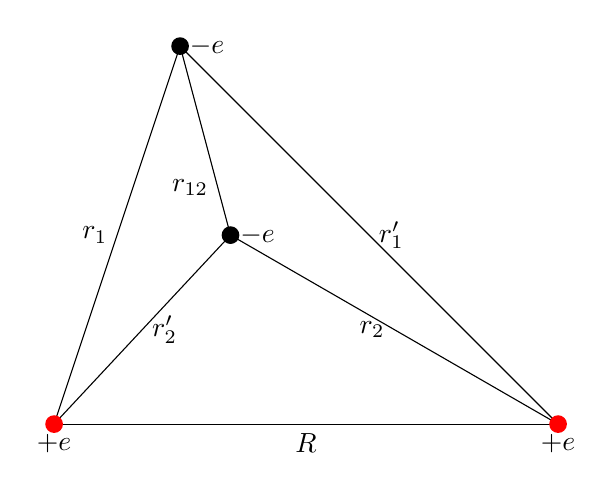
\begin{tikzpicture}[scale=0.8]
            % 定点
            \coordinate [label=below:$+e$] (A) at (0,0);
            \coordinate [label=below:$+e$] (B) at (8,0);
            \coordinate [label=right:$-e$] (C) at (2,6);
            \coordinate [label=right:$-e$] (D) at (2.8,3.0);
            % 画线 % 标记线段
            \draw (A) -- (B) node[midway,below]{$R$};
            \draw (B) -- (C) node[midway,right]{$r_1^\prime$};
            \draw (C) -- (A) node[midway,left]{$r_1$};
            \draw (D) -- (A) node[midway,right]{$r_2^\prime$};
            \draw (D) -- (B) node[midway,left]{$r_{2}$};
            \draw (D) -- (C) node[near start,left]{$r_{12}$};
            % 画粒子图示
            \foreach \point in {C,D}
                \fill [black,opacity=1] (\point) circle (4pt);
            \foreach \point in {A,B}
                \fill [red,opacity=1] (\point) circle (4pt);
        \end{tikzpicture}
        \caption{$\ce{H2}$图示, 黑点表示电子, {\color{red} 红点}表示质子}
        \label{fig:8.1}
    \end{figure}
    
    我们很自然地首先根据一个电子在两个质子作用下的轨道近似\ref{eq:8.12}得到两个电子的轨道或许具有下面的形式:
    \begin{equation}
        \begin{aligned}
            \psi\left(\mathbf{r}_{1}, \mathbf{r}_{2}\right)&=A\left[{\psi_{0}\left(r_{1}\right)+\psi_{0}\left(r_{1}^{\prime}\right)}\right]\left[{\psi_{0}\left(r_{2}\right)+\psi_{0}\left(r_{2}^{\prime}\right)}\right]\\
            &=A\left[\psi_{0}\left(r_{1}\right) \psi_{0}\left(r_{2}^{\prime}\right)+\psi_{0}\left(r_{1}^{\prime}\right) \psi_{0}\left(r_{2}\right)+\cancel{\psi_{0}\left(r_{1}\right) \psi_{0}\left(r_{2}\right)}+\cancel{\psi_{0}\left(r_{1}^{\prime}\right) \psi_{0}\left(r_{2}^{\prime}\right)}\right]
        \end{aligned}
    \end{equation}
    
    后面两项我们不要是因为考虑到电子之间有斥力, 而后面两项对应这两个电子相对于同一个质子的轨道耦合, 而根据电子之间的排斥, 两电子相对于同一个质子的轨道之间的耦合
    应当是微乎其微的, 所以我们要保留的应当是两个电子相对于不同质子之间轨道的耦合。
    \[\psi_{+}\left(\mathbf{r}_{1}, \mathbf{r}_{2}\right)=A_{+}\left[\psi_{0}\left(r_{1}\right) \psi_{0}\left(r_{2}^{\prime}\right)+\psi_{0}\left(r_{1}^{\prime}\right) \psi_{0}\left(r_{2}\right)\right]\]
    
    上面的是对称的波函数, 电子是费米子, 实际上这说明电子的自旋是singlet, 当然, 这也意味着还有一种自旋为triplet所对应的反对称波函数:
    \[\psi_{-}\left(\mathbf{r}_{1}, \mathbf{r}_{2}\right)=A_{-}\left[\psi_{0}\left(r_{1}\right) \psi_{+}\left(r_{2}^{\prime}\right)+\psi_{0}\left(r_{1}^{\prime}\right) \psi_{0}\left(r_{2}\right)\right]\]
    
    这两个试探波函数\footnote{化学家称之为\textbf{Heitler-London近似}}都有一定道理, 因为我们并不能事先知道电子到底选取的是何种自选耦合, 所以现在我们两个一起考虑。首先进行归一化:
    \begin{equation}
        \begin{aligned}
            1= & \iint\left|\psi_{\pm}\left(\mathbf{r}_{1}, \mathbf{r}_{2}\right)\right|^{2} d^{3} \mathbf{r}_{1} d^{3} \mathbf{r}_{2} \\
            = & A_{\pm}^{2}\left[\int \psi_{0}\left(r_{1}\right)^{2} d^{3} \mathbf{r}_{1} \int \psi_{0}\left(r_{2}^{\prime}\right)^{2} d^{3} \mathbf{r}_{2}+\int \psi_{0}\left(r_{1}^{\prime}\right)^{2} d^{3} \mathbf{r}_{1} \int \psi_{0}\left(r_{2}\right)^{2} d^{3} \mathbf{r}_{2}\right. \\
            & \left.\pm 2 \int \psi_{0}\left(r_{1}\right) \psi_{0}\left(r_{1}^{\prime}\right) d^{3} \mathbf{r}_{1} \int \psi_{0}\left(r_{2}^{\prime}\right) \psi_{0}\left(r_{2}\right) d^{3} \mathbf{r}_{2}\right]
        \end{aligned}
    \end{equation}
    括号内前面两项是1后面一项实际上是$I^2$(cf.\ref{eq:8.14})。得到归一化因子:
    \begin{equation}
        A_{\pm}=\frac{1}{\sqrt{2\left(1 \pm I^{2}\right)}}
    \end{equation}
    再根据\ref{eq:8.15}:
    \begin{equation}
        \begin{aligned}
            -\frac{\hbar^{2}}{2 m} \nabla_{1}^{2} \psi_{\pm}= & A_{\pm}\left[\left(-\frac{\hbar^{2}}{2 m} \nabla_{1}^{2} \psi_{0}\left(r_{1}\right)\right) \psi_{0}\left(r_{2}^{\prime}\right) \pm\left(-\frac{\hbar^{2}}{2 m} \nabla_{1}^{2} \psi_{0}\left(r_{1}^{\prime}\right)\right) \psi_{0}\left(r_{2}\right)\right] \\
            = & A_{\pm}\left[\left(E_{1}+\frac{e^{2}}{4 \pi \epsilon_{0} r_{1}}\right) \psi_{0}\left(r_{1}\right) \psi_{0}\left(r_{2}^{\prime}\right) \pm\left(E_{1}+\frac{e^{2}}{4 \pi \epsilon_{0} r_{1}^{\prime}}\right) \psi_{0}\left(r_{1}^{\prime}\right) \psi_{0}\left(r_{2}\right)\right] \\
            = & E_{1} \psi_{\pm}+\frac{e^{2}}{4 \pi \epsilon_{0} a} A_{\pm}\left(\frac{a}{r_{1}} \psi_{0}\left(r_{1}\right) \psi_{0}\left(r_{2}^{\prime}\right) \pm \frac{a}{r_{1}^{\prime}} \psi_{0}\left(r_{1}^{\prime}\right) \psi_{0}\left(r_{2}\right)\right) 
        \end{aligned}
    \end{equation}
    根据\ref{eq:8.17}、\ref{eq:8.19}一通计算后:
    \begin{equation}
        \Braket{-\frac{\hbar^{2}}{2 m} \nabla_{1}^{2}}=E_{1}+\left(\frac{e^{2}}{4 \pi \epsilon_{0} a}\right) \frac{1 \pm I X}{1 \pm I^{2}}=\Braket{-\frac{\hbar^{2}}{2 m} \nabla_{2}^{2}}
    \end{equation}
    又是一个繁琐但是类似的计算, 我们可以得到:
    \begin{equation}
        \left\langle-\frac{e^{2}}{4 \pi \epsilon_{0} r_{1}}\right\rangle=-\frac{1}{2}\left(\frac{e^{2}}{4 \pi \epsilon_{0} a}\right) \frac{1+D \pm 2 I X}{1 \pm I^{2}}
    \end{equation}
    最后, 来计算一下电子之间的库伦势:
    \begin{equation}
        \braket{V_{ee}}\equiv\Braket{\frac{e^2}{4\pi\varepsilon_0}r_{12}}=\left(\frac{e^2}{4\pi\varepsilon_0}\right)\frac{D_2\pm X_2}{1\pm I^2}
    \end{equation}
    其中:
    \begin{equation}
        \begin{aligned}
            &D_{2}=\iint\left|\psi_{0}\left(r_{1}\right)\right|^{2} \frac{a}{r_{12}}\left|\psi_{0}\left(r_{2}^{\prime}\right)\right|^{2} d^{3} \mathbf{r}_{1} d^{3} \mathbf{r}_{2} \\
            &X_{2}=\iint \psi_{0}\left(r_{1}\right) \psi_{0}\left(r_{1}^{\prime}\right) \frac{a}{r_{12}} \psi_{0}\left(r_{2}\right) \psi_{0}\left(r_{2}^{\prime}\right) d^{3} \mathbf{r}_{1} d^{3} \mathbf{r}_{2}
        \end{aligned}
    \end{equation}

    第一个的物理意义非常明显, 就是电荷体密度分布分别为$\rho_1=|\psi_0(\mathbf{r}_1)|$和$\rho_2=|\psi_0(\mathbf{r}_2)|$的带电体之间的电势能, 这次给化学家说中了, 
    就好像是两坨电子云相互作用。这个积分也相对好算一点, 只用注意到现在$\mathbf{r}_1$和$\mathbf{r}_2$之间相互独立, 要作两次三重积分, 结果为:
    \begin{equation}
        D_{2}=\frac{a}{R}-e^{-2 R / a}\left[\frac{1}{6}\left(\frac{R}{a}\right)^{2}+\frac{3}{4}\left(\frac{R}{a}\right)+\frac{11}{8}+\frac{a}{R}\right]
    \end{equation}
    但是另一个那就是真的难搞了, 详细计算戳这篇文献\footnote{\url{https://doi.org/10.1007/BF01329207}, 但是很不幸, 原始文献是德文的。}:
    \begin{equation}
        \begin{aligned}
            X_{2}= & e^{-2 R / a}\left[\frac{5}{8}-\frac{23}{20} \frac{R}{a}-\frac{3}{5}\left(\frac{R}{a}\right)^{2}-\frac{1}{15}\left(\frac{R}{a}\right)^{3}\right] \\
            & +\frac{6}{5} \frac{a}{R} I^{2}\left[\gamma+\log \left(\frac{R}{a}\right)+\left(\frac{\tilde{I}}{I}\right)^{2} \mathrm{Ei}\left(-\frac{4 R}{a}\right)-2 \frac{\tilde{I}}{I} \mathrm{Ei}\left(-\frac{2 R}{a}\right)\right]
        \end{aligned}
    \end{equation}
    其中$\gamma=0.5772\ldots$是Euler常数, 
    \[\operatorname{Ei}(x)\equiv -\int_{-x}^{\infty} \frac{e^{-t}}{t} d t,\quad\tilde{I}\equiv e^{R / a}\left[1-\frac{R}{a}+\frac{1}{3}\left(\frac{R}{a}\right)^{2}\right]\]
    最后我们加上质子之间的势能:
    \begin{equation}
        E_{gs}\leq\braket{H}_{\pm}=2 E_{1}\left[1-\frac{a}{R}+\frac{2 D-D_{2} \pm\left(2 I X-X_{2}\right)}{1 \pm I^{2}}\right]
    \end{equation}
    
    画出$\braket{H}_\pm$的图像\ref{fig:8.2}后可以发现, singlet对应的能量更小, 所以电子更倾向于采取$\psi_+$的轨道。和上一小节类似, 我们可以计算出对应的键长$\SI[]{0.87}{\angstrom}$(实验值$\SI[]{0.74}{\angstrom}$)
    , 键能$\SI[]{3.15}{eV}$(实验值$\SI[]{4.75}{eV}$)。
    \begin{figure}[htbp]
        \centering
        \includegraphics[scale=0.8]{fig/8-2.eps}
        \caption{$\braket{H}_\pm$的图像, 虚线表示$\braket{H}_-$, 实线表示$\braket{H}_+$}
        \label{fig:8.2}
    \end{figure}